%%%%%%%%%%%%%%%%%%%%%%%%%%%%%%%%%%%%%%% Titelseite
%\titlehead{
%\begin{center}
%\vspace{-2cm}
%
\includegraphics[scale=0.27]{Bilder/Otto.png} \\
%\end{center}
%}
\titlehead{
\vspace{-2cm}
\begin{center}
 
\includegraphics[scale=2]{Bilder/Otto_neu.eps}
\end{center}
\vspace{1cm}
}
\subject{\LARGE Masterarbeit\vspace{-5mm}}
\title{\huge Lighthouse Keeper \\ \LARGE Ein neues Verfahren für Indoor-Lokalisierung \\ mit adaptiven iBeacon Konfigurationen\\
\vspace{1mm}
\textnormal{\small von}\vspace{-1cm}}
\author{\textnormal{\large André Pieper} \\[-3mm] \textnormal{\large Geb. 28.03.1988 in Berlin} \\[-3mm] \textnormal{\large Matrikelnummer: 184960} \vspace{0.5cm}}
\date{31. März 2015}
\publishers{
\begin{figure}[h]
$\begin{minipage}[b]{13cm}
	\vspace{0.5cm}
	\begin{normalsize}
	\begin{tabular}[h]{ll}
	Erstprüfer: & Jun.-Prof. Dr.-Ing. Sebastian Zug \\
	& Otto-von-Guericke-Universität \\
	& Fakultät für Informatik \\
	& Institut für Verteilte Systeme \\
	& Lehrstuhl Embedded Smart Systems \\
	& Universitätsplatz 2, D-39106, Magdeburg \\ \\

	Zweitprüfer: & Prof. Dr.-Ing. Abbas Omar \\
	& Otto-von-Guericke-Universität \\
	& Fakultät für Elektro- und Informationstechnik \\
	& Institut für Informations- und Kommunikationstechnik\\
	& Lehrstuhl für Hochfrequenz- und Kommunikationstechnik \\
	& Universitätsplatz 2, D-39106, Magdeburg 
	\end{tabular}
	\vspace{-2cm}
	\end{normalsize}
\end{minipage}
\begin{minipage}[b]{3cm}
\begin{flushright}
 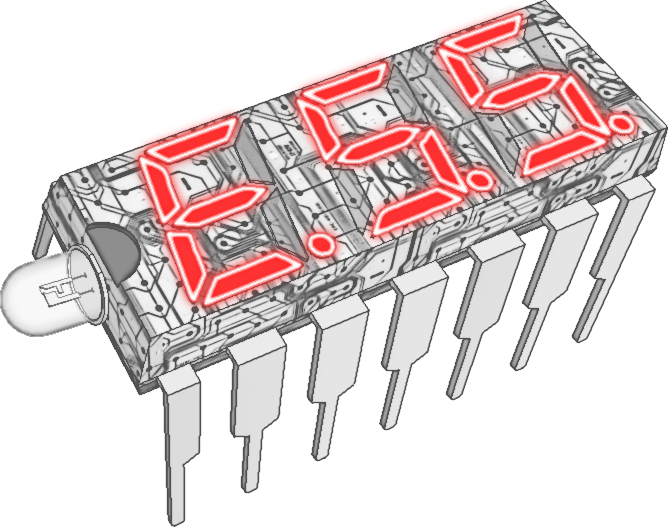
\includegraphics[scale=0.2]{Bilder/ESS.png} \\[2.5cm]
 
\includegraphics[scale=0.2]{Bilder/IIKT.png}
\end{flushright}
\end{minipage}$
\end{figure}
}

\begin{document}
\maketitle 
\newpage\thispagestyle{empty}~
\newpage
\setcounter{tocdepth}{2}

\section*{Kurzdarstellung}
Satellitengestütze Navigationssysteme sind in der heutigen Zeit ein fester Bestandteil des alltäglichen Lebens. Sie ermöglichen zum Beispiel die Orientierung eines Autofahrers auf für ihn fremden Straßen und sind mittlerweile serienmäsig in Autos, Smarphones und sogar Kameras intigriert. Aber die Signale der satellitengestützten Lokalisierungs-Systeme wie GPS, GLONASS und Galileo verlieren sich in Gebäuden, da sie durch deren Strukturen absorbiert, bzw. reflektiert werden. Dabei soll, so wie die "`Outdoor"'-Lokalisierungssysteme den Straßenverkehr revolutionierten, ein neues "`Indoor"'-System das Vorankommen von Menschen in Gebäuden verändern: die iBeacons. Während es viele Unternehmen gibt, die diese Technik bereits herstellen und vermarkten, gibt es jedoch noch keine zufriedenstellende Strategie, die nötige Infrastruktur für ein Lokalisierungssystem aus iBeacons effizient zu planen und zu testen. Gegenstand dieser Arbeit soll es sein, ein mögliches Verfahren dafür zu entwickeln und sich dabei verstärkt auf Automation mithilfe von Robotern zu konzentrieren, um das Potential dieser jungen Technologie weiter auszuschöpfen.  